\documentclass{elsarticle}
\usepackage[margin=1.25in]{geometry}
\usepackage[utf8]{inputenc}
\usepackage{todonotes}
\usepackage{parskip}
\usepackage{amsmath}
\usepackage{amssymb}
\usepackage{ulem}

\graphicspath{ {./Figures/} }

%\usepackage[numbers,sort&compress]{natbib}
\bibliographystyle{elsarticle-num}

\title{Li-Sulfur Modeling}

\begin{document}

\maketitle

%===============================================================%
%                       INTRODUCTION
%===============================================================%
\section{Introduction}
The growing push for decarbonization has lead to exploring better balances of energy production and storage. In order to accommodate energy storage that helps shift energy production, batteries with higher capacity, energy density, power density, and lifespan all while providing safer and cheaper alternatives to current technology, are necessary. Lithium-sulfur batteries are a promising “beyond Li-ion” battery technology, leveraging the high specific capacity (approximately 1675 Ah/kg$_\mathrm{sulfur}$) and the natural abundance of sulfur to produce lighter, cheaper batteries for portable applications. Despite promising theoretical capacity, commercialization of lithium-sulfur batteries is limited by inherent material properties which reduce battery performance and durability. The primary material properties of concern are the low conductivities of the charge and discharge end-states (S$_8$ and Li$_2$S), volumetric expansion during discharging from S$_8$ to Li$_2$S, and the low reduction potential of sulfur and lithium polysulfide intermediates, relative to Li/Li$^+$ \cite{ZHANG2018831, FRONCZEK2013183, C5EE01388G}. In addition, the solubility of some intermediate species and insolubility of others adds cell design and operation concerns that need to be considered. The low discharge voltages, the need for an electronically conductive host network, and high electrolyte/sulfur ratios, reduce typical Li-S battery energy and power densities well below their theoretical values \cite{BRUCKNER201482, akridge2004}.

Of the challenges faced for lithium-sulfur batteries, polysulfide shuttling is affected by both design and operation parameters and is a far-reaching problem. Due to this, much of the current research on lithium-sulfur batteries is focused on either preventing the dissolution of the intermediate products into the electrolyte or preventing their migration to the anode \cite{CHEN20201605, liu2016, cheng2019, pang2015}. Polysulfide shuttling occurs when soluble intermediate species that form during discharge of the battery move between the anode and the cathode \cite{C5EE01388G}. At the anode these intermediate order polysulfides (Li$_2$S$_x$) can react and be further reduced. If low order polysulfides (x $<$ 3) are formed isolated from the electronically conductive carbon network of the cathode, they become lost active material and result in capacity fade of the battery. There are concurrent efforts to reduce the electrolyte/sulfur ratio to maximize the battery’s gravimetric energy density. However, for any of these strategies, it is critical to understand and control the intermediate species concentrations in the electrolyte, both to optimize performance and to minimize capacity fade due to precipitation of species which exceed their solubility limits. The solubility of intermediate products varies slightly with the electrolyte used, but they trend downward as the polysulfide order decreases.

This paper builds on previous modeling efforts, starting with the 1-D model developed by Kumaresan \textit{et al} \cite{Kumaresan_2008}. Other models have followed to look at things such as transport limitations \cite{ZHANG2016502}, impedance spectra \cite{FRONCZEK2013183}, polysulfide shuttling and capacity loss \cite{HOFMANN2014300}, and nucleation and growth mechanisms in lithium sulfur cells \cite{REN2016115}. The standard reaction mechanism for these models is a linear chain of reactions proceeding from S$_8$ to Li$_2$S with no side reactions, disproportionation, or association reactions. The model presented here will start from this type of linear reaction mechanism while incorporating physically derived parameters to capture the evolution of the cathode morphology throughout the discharge and charge processes. Then the model will further implement reaction mechanisms derived from studies that use DFT and quantum chemical calculations to obtain reaction and species thermodynamics as well as theoretical reduction potentials of species \cite{assary2014, kuzmina2019}. The model is built in such a manner to allow for flexible use of various electrochemical mechanisms with the same physical model of the lithium-sulfur cell. Thus, mechanisms of varying complexity can be compared directly with relative ease. In addition to a comparison of mechanisms, the model will be used to explore other aspects of lithium-sulfur batteries, such as electrolyte/sulfur ratio, cathode porosity, and energy versus power density with solubility considerations.




%===============================================================%
%                       BACKGROUND
%===============================================================%
\section{Background}

(Discuss problems we are trying to solve/understand, previous modeling efforts/literature review, and availability of validation data).




%===============================================================%
%                       MODEL FORMULATION
%===============================================================%

\section{Model Formulation}
The model presented herein is written as a set physically-derived conservation equations, discretized in one dimension using a finite volume approach, and integrated as a function of time during galvanostatic discharge and charge of the single-cell battery.  The model equations implement conservation of mass, elements, and charge, and taken together constitute a set of differential algebraic equations.  The model is written in python, using the software package Assimulo \cite{assimulo} to integrate the DAE set, and using \textsc{Cantera} \cite{cantera} to calculate and manage species and phase thermochemical calculations. In this section, we present the model formulation, including relevant conservation equations, boundary and initial conditions, and model parameters, including thermo-kinetic mechanism properties and microstructural geometric parmeters.

\subsection{Model Domain}

In lithium-sulfur batteries, the cathode is composed of a conductive host material, typically carbon based, in which the sulfur is infiltrated by melt infiltration or chemical vapor deposition \cite{BRUCKNER201482}. The model presented here will represent the cathode domain as a series of representative carbon particles with some surface area on which representative hemispherical particles of the solid products that form during dis/charge as shown in Fig. \ref{fig:modeldomain}. The model currently models three solid phases in the cathode: carbon, sulfur, and lithium sulfide. Due to the significant volumetric expansion that occurs during discharge of these batteries, the pore space will change as well. Currently, the model assumes the total cell volume remains constant through dis/charge. This requires the effect on species concentration in the electrolyte to be accounted for in the conservation equations. During discharge, the solid sulfur dissolves into the electrolyte where it can be reduced at the carbon/electrolyte interface to form lithium polysulfides. These polysulfides can be further reduced at the carbon/electrolyte interface or the lithiumsulfide/carbon/electrolyte three phase boundary (tpb) once the lithium sulfide begins to form. The anode is treated as an ideal lithium metal anode that acts as the reservoir for Li+ in the cell. At the current collector for both electrodes, a constant current boundary condition is imposed during discharge and charge. 

\begin{center}
\begin{figure}
    \centering
    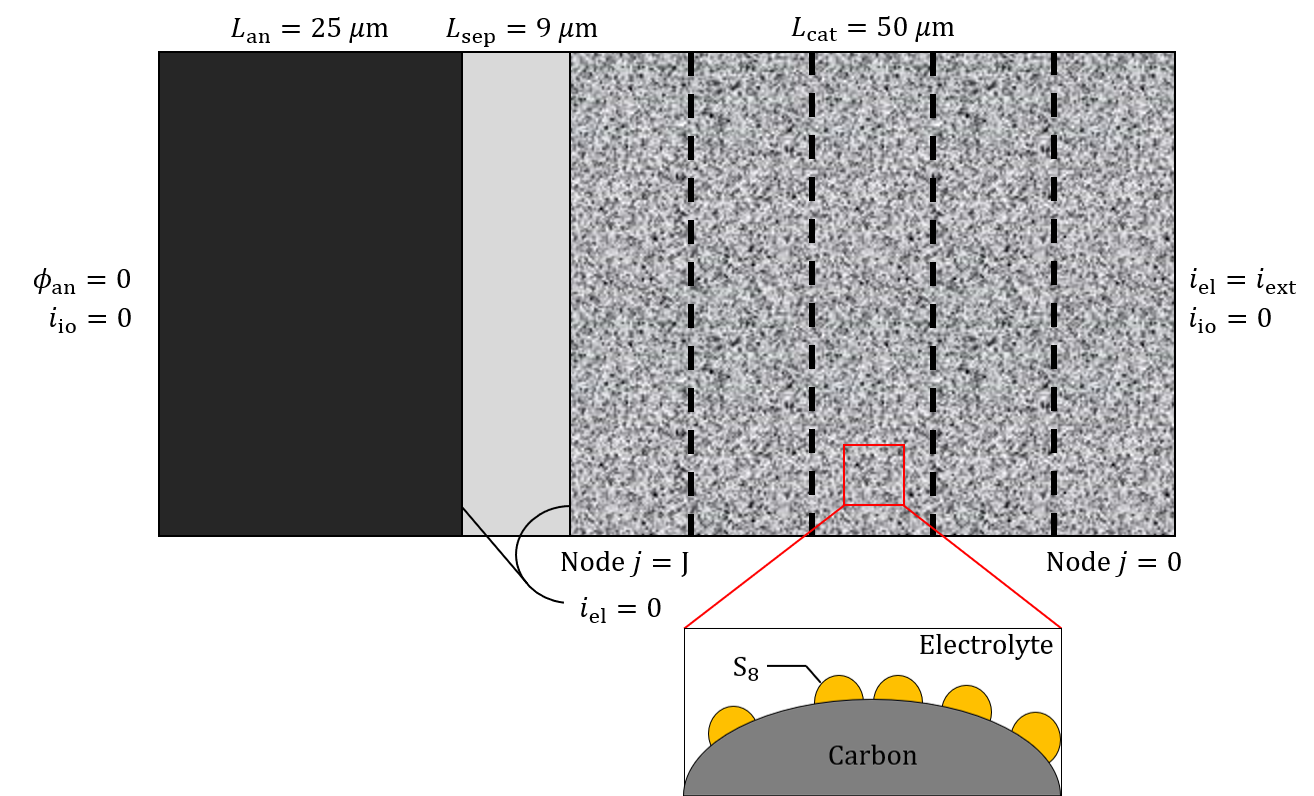
\includegraphics[width=\textwidth]{model_domain.png}
    \caption{Caption}
    \label{fig:modeldomain}
\end{figure}
\end{center}

\subsection{Governing Equations}
The battery’s state at any given location and point in time is fixed by the following variables:

In the cathode:
\begin{itemize}
    \item $\varepsilon_{\rm S_8}$, volume fraction of solid sulfur (-)
	\item $\varepsilon_{\rm Li_2S}$, volume fraction of lithium sulfide (-)
	\item $C_{k,\,{\rm elyte}}$, molar concentration of species $k$ in the electrolyte phase $\left({\rm kmol}_k\, {\rm m_{elyte}^{-3}}\right)$
	\item $\phi_{\rm carbon}$, the electric potential of the cathode carbon phase (V)
	\item $\phi_{\rm elyte}$, the electric potential of the electrolyte phase (V)
\end{itemize}

In the electrolyte separator:
\begin{itemize}
    \item $C_{k,\,{\rm elyte}}$, molar concentration of species $k$ in the electrolyte phase $\left({\rm kmol}_k\, {\rm m_{elyte}^{-3}}\right)$
    \item $\phi_{\rm elyte}$, the electric potential of the electrolyte phase (V)
\end{itemize}

In the anode:
\begin{itemize}
    \item $\phi_{\rm Li}$, the electric potential of the metallic Li anode phase (V)
\end{itemize}

The evolution of these variables during battery operation is predicted via governing equations derived from physically-based conservation equations for the mass, elements, and electrical charge:

\subsubsection{Solid Phase Volume Fractions}
For the cathode solid-phase end states--solid sulfur S$_8$ in the charged state and solid Li$_2$S in the discharged state--constant mass density is assumed for all species in the phase. As such, conservation of mass leads to the following for $\varepsilon_m$, the volume fraction of a solid phase $m$: 

\begin{equation}\label{eq:dEps_dt}
    \frac{\partial \varepsilon_m}{\partial t} = a_m\sum_{k,\,m} \overline{v}_k\dot{s}_k,
\end{equation}
where $\overline{v}_k$ is the constant molar volume (m$^3$ kmol$^{-1}$, equal to the molar mass divided by the mass density) and $\dot{s}_k$ the molar production rate due to heterogeneous surface reactions (kmol$_k$ m$^{-2}$ s$^{-1}$) for species $k$, summed over all $k$ species in phase $m$.  The parameter $a_m$ is the volume-specific area of the reactio interface between the phase $m$ and the electrolyte.

\subsubsection{Electrolyte Species}
The molar concentration of the electrolyte species in the porous regions of the cathode and electrolyte separator will vary with time due to processes including chemical and electrochemical reactions, species transport, and the change in electrolyte volume fraction due to changing solid phase volume fractions. Conservation of mass and elements are combined to derive the following differential equation for the evolution of the species molar concentrations $C_{k,\,{\rm elyte}}$  (kmol m$_{\rm elyte}^{-3}$):
\begin{equation}\label{eq:dCkelyte_dt}
    \frac{\partial C_{k,\,{\rm elyte}}}{\partial t} = \frac{1}{\varepsilon_{\rm elyte}}\left(\sum_m a_m\dot{s}_{k,\,{\rm elyte}} + \dot{\omega}_{k,\,{\rm elyte}} - \nabla N_{k,\,{\rm elyte}}\right) - C_{k,\,{\rm elyte}}\frac{\partial \varepsilon_{\rm elyte}}{\partial t},
\end{equation}

where $\dot{\omega}_{k,\,{\rm elyte}}$ is is molar production rate of electrolyte species $k$ due to homogeneous electrolyte phase reactions (kmol m$^{-3}$ s$^{-1}$),and $N_{k,\,{\rm elyte}}$ is the molar flux of electrolyte species $k$ (kmol m$^{-2}$ s$^{-1}$) in the $z$ direction. There are no surface reactions in the electrolyte separator ($a_m\dot{s}_{k,\,{\rm elyte}} = 0$), and homogeneous reactions are neglected throughout the modeling domain ($\dot{\omega}_{k,\,{\rm elyte}}=0$), at present. The rate of change of the electrolyte volume fraction $\left(\frac{\partial \varepsilon_{\rm elyte}}{\partial t}\right)$ is calculated as:
\begin{equation}\label{eq:dEpsElyte_dt}
    \frac{\partial \varepsilon_{\rm elyte}}{\partial t} = -\frac{\partial \varepsilon_{\rm S_8}}{\partial t} -\frac{\partial \varepsilon_{\rm Li_2S}}{\partial t},
\end{equation}
where the solid phase volume fraction rates of change are calculated as in eq.~\ref{eq:dEps_dt}, above.

\subsubsection{Phase Electric Potentials}
 Within the cathode, the electrolyte and cathode carbon phase electric potentials are solved by applying conservation of charge and assuming charge neutrality. Charge neutrality in the electrolyte phase of a given volume implies that the sum of all currents into the volume equals zero:

 \begin{equation}\label{eq:ChargeCons_elyte}
     0 = \nabla i_{\rm io} + i_{\rm Far} + i_{\rm dl},
 \end{equation}
where $i_{\rm io}$ is the ionic electrolyte phase current density ${\rm \left(A\,cm^{-2}\right)}$, $i_{\rm Far}$ is the local Faradaic charge transfer current per unit volume ${\rm \left(A\,cm^{-3}\right)}$, and $i_{\rm dl}$ is the local double-layer current per unit volume ${\rm \left(A\,cm^{-3}\right)}$.  $i_{\rm Far}$ and $i_{\rm dl}$ are formulated such that positive current represents net positive charge transferred from the electrolyte phase to the carbon phase. The currents in eq.~\ref{eq:ChargeCons_elyte} are illustrated schematically in Fig. \ref{fig:currentdiagram}. 

\begin{center}
\begin{figure}
    \centering
    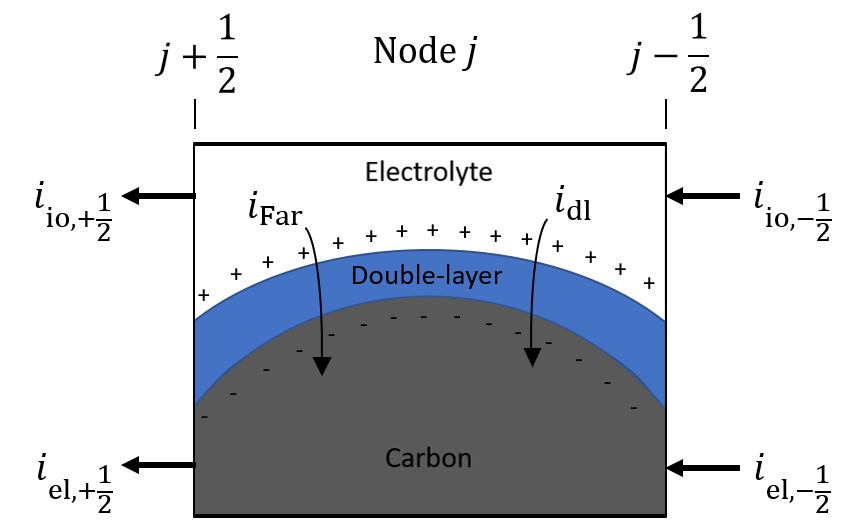
\includegraphics[width=\textwidth/2]{CurrentDiagram.png}
    \caption{Caption}
    \label{fig:currentdiagram}
\end{figure}
\end{center}

The ionic current in the electrolyte is a function of the species fluxes $N_{k,\,{\rm elyte}}$:
\begin{equation}\label{eq:i_io}
    i_{\rm io} = F\sum_{k,{\rm elyte}} z_kN_{k},
\end{equation}
where $F$ is Faraday's constant and $z_k$ is the elementary charge of species $k$. The double layer current, therefore, balances the residual of the sum of the remaining charges, transferring charge between the electrolyte bulk phase and the capacitive double layer at the electrolyte/carbon interface to maintain charge neutrality in the electrolyte bulk. Modeling the double layer as a capacitor with capacitance $C_{\rm dl}$ (F m$^{-2}$) links the rate of change of the double layer potential $\Delta \phi_{\rm dl}$ to the double-layer current:
\begin{equation}\label{eq:ddPhi_dt}
    \frac{\partial \Delta \phi_{\rm dl}}{\partial t} = \frac{i_{\rm dl}}{C_{\rm dl}\,a_{\rm dl}},
\end{equation}
where the double layer potential equals the difference between the cathode carbon phase and the bulk electrolyte phase:
\begin{equation}\label{eq:dPhi_dl}
    \Delta \phi_{\rm dl} = \phi_{\rm ca} - \phi_{\rm elyte},
\end{equation}
where $\phi_{\rm ca}$ and $\phi_{\rm elyte}$ are the cathode carbon and electrolyte electric potentials, respectively. Conservation of charge and charge neutrality are also applied to teh cathode volume as a whole (electronically conducting cathode + ionically conducting electrolyte phases) to yield:
\begin{equation}\label{eq:ChargeCons_tot}
    0 = \nabla i_{\rm io} + \nabla i_{\rm el},
\end{equation}
where $i_{\rm el}$ is the electronic carbon-phase current density $\left({\rm A\,cm^{-2}} \right)$. As documented below, $i_{\rm io}$ is a function of $C_{k,\,{\rm elyte}}$ and $\phi_{\rm elyte}$, while the electronic current is a function of $\phi_{\rm ca}$ only.  Eqs.~\ref{eq:ddPhi_dt}--~\ref{eq:ChargeCons_tot} therefore fix the electric potentials of the two phases throughout the domain. Eq.~\ref{eq:ddPhi_dt} represents a differential equation which is integrated in time to solve the double layer potential. $\Delta \phi_{\rm dl}$ is, in turn, used to calculate the $\phi_{\rm elyte}$ at any given time via eq.~\ref{eq:dPhi_dl}. Eq.~\ref{eq:ChargeCons_tot}, meanwhile, is an algebraic equation that must be satisfied at any point in time by the cathode carbon phase electric potentials. 

In the electrolyte separator, there is no electronic current, and so eq.~\ref{eq:ChargeCons_tot} reduces to:
\begin{equation}
    0 = \nabla i_{\rm io},
\end{equation}
with $i_{\rm io}$ calculated as in eq.~\ref{eq:i_io}.

The anode is modeled as a dense Li foil, and as such the electric potential of the anode is resolved via a capacitive double layer at the electrolyte separator--anode boundary.  Charge neutrality in the anode requires that all currents sum to zero:
\begin{equation}\label{eq:ChargeConsAnode}
    i_{\rm ext} + i_{\rm Far,\,an} + i_{\rm dl,\,an} = 0,
\end{equation}
where all currents represent positive charge delivered to the bulk Li anode.  $i_{\rm ext}$ represents the user-specific external current (positive current corresponds to battery discharge).  As with the cathode, $i_{\rm dl}$ is used to calculate the rate of change of the anode--electrolyte double layer potential, via eq.~\ref{eq:ddPhi_dt}.


\subsection{Process Variables: Reaction and Transport Rate Calculations}

The charge-transfer reactions are evaluated using mass action kinetics, and are handled by \textsc{Cantera}. The \textsc{Cantera} input file allows user specification of Arrhenius parameters (pre-exponential $A$, temperature exponent $b$, and activation energy $E_{\rm a}$) for the forward rate coefficient:
\begin{equation}\label{eq:k_fwd_echem}
    k_{\rm f} = AT^b\exp\left(-\frac{E_{|rm a}}{RT}\right)\exp\left(-\sum_k\frac{\beta\nu_kz_k\phi_k}{RT}\right).
\end{equation}
Here, $R$ is the universal gas constant, $T$ the temperature, $\beta$ the charge-transfer symmetry factor, and $\nu_k$, $z_k$, and $\phi_k$ are the net stoichiometric coefficient, elementary charge, and electric potential of the phase for species $k$, respectively.  For non-charge-transfer reactions, the electric potential summation evaluates to zero, and typical Arrhenius rate coefficients are recovered.  The reverse rate coefficient $k_{\rm r}$ for the same reaction is calculated as the reaction's equilibrium coefficient, divided by the forward rate coefficient, to maintain thermodynamic consistency \cite{DeCaluwe_2018}.

For a reaction $i$, the net rate of progress $\dot{q}_i$ is
\begin{equation}\label{eq:rop_net}
    \dot{q}_i = k_{{\rm f},i}\prod_k C_{{\rm ac},\,k}^{\nu^\prime_{k,i}} -  k_{{\rm r},i}\prod_k C_{{\rm ac},\,k}^{\nu^{\prime\prime}_{k,i}},
\end{equation}
where $\nu^\prime_{k,i}$ and  $\nu^{\prime\prime}_{k,i}$ are the forward and reverse stoichiometric coefficients for species $k$ in reaction $i$, respectively, and $C_{{\rm ac},\,K}$ is the ``activity concentration'' for species $k$ (equal to the molar density times the activity coefficient).  Finally, the net production rate for a given species due to a set of reactions ($\dot{s}_k$ or $\dot{\omega}_k$, above; we will use $\dot{s}_k$, here, for demonstration purposes) is:
\begin{equation}\label{eq:net_prod_rate}
    \dot{s}_k = \sum_i \nu_{k,i}\dot{q}_i.
\end{equation}
Transport rate calculations for electrolyte species use the Nernst-Poisson-Planck formulation and the dilute solution approximation:
\begin{equation}\label{eq:PNP}
    N_{k,{\rm elyte}} = -D_k^{\rm eff}\left(\nabla C_k + C_k\frac{z_kF}{RT}\nabla \phi_{\rm elyte}\right),
\end{equation}
where $C_k$ is taken at the interface between adjacent volumes (via weighted averaging of the volume-center concentrations). $D^{\rm eff}_k$ the effective diffusion coefficient, which incorporates the local microstructure (which varies dynamically in the cathode):
\begin{equation}\label{eq:Dk_eff}
    D^{\rm eff}_k = \frac{\varepsilon}{\tau_{\rm fac}}D^\circ_k = D^\circ_k\varepsilon^{1.5}
\end{equation}
where the bulk diffusion coefficient (absent microstructure impacts) is $D^\circ_k$, and where we replace the local tortuosity factor $\tau_{\rm fac}$ with a simple Bruggeman correlation, $n_{\rm Bruggeman} = -0.5$ \cite{TJADEN201644}.  Although eq.~\ref{eq:PNP} can accommodate the more accurate concentrated solution theory (CST) \cite{Kupper_2016}, the CST framework requires significant alteration to accomodate the multiple charged species in the Li-S system \cite{mukherjee2018}, and is left for future work.
\subsection{Initial Conditions and Geometric Parameters}
A novel feature of this model is the use of physically derived geometric parameters, such as specific surface area, which directly links model microstructural parameters to  battery design and fabrication parameters from reported experiments. Here, we describe the derivation of  microstructural parameters from a small number of experimental/cell fabrication variables and physical constants:
\begin{itemize}
    \item $m^{\prime\prime,\circ}_{\rm S_8}$, the initial mass loading of sulfur (kg m$^{-3}$)
    \item $m^\circ_{\rm S_8}$, the initial bulk mass of sulfur (kg)
    \item $\omega^\circ_m$, the area-specific weight percent of each phase $m$ (kg$_m$ kg$^{-1}_{\rm tot}$ m$^{-2}$)
    \item $H_{\rm ca}$, the cathode thickness (m)
    \item $\rho_m$, the mass density of phase $m$, (kg$_m$ m$^{-3}_m$)
\end{itemize}
These input parameters allow calculation of the initial volume fraction of solid phases:
\begin{equation}\label{eq:esp_S8_o}
    \varepsilon_{\rm S_8}^\circ = \frac{m^{\prime\prime,\circ}_{\rm S_8}}{\rho_{\rm S_8} H_{\rm ca}}
\end{equation}
\begin{equation}\label{eq:m_solid_o}
    m^\circ_{\rm solid} = \frac{m^{\prime\prime,\circ}_{\rm S_8}}{\omega^\circ_{\rm S_8}}
\end{equation}
\begin{equation}\label{eq:eps_carbon_o}
    \varepsilon^\circ_{\rm carbon} = \frac{ m^\circ_{\rm solid}\omega^\circ_{\rm carbon}}{\rho_{\rm carbon}H_{\rm ca}}
\end{equation}
\begin{equation}\label{eq:eps_elyte_o}
    \varepsilon^\circ_{\rm elyte} = 1 - \varepsilon^\circ_{\rm S_8} - \varepsilon^\circ_{\rm carbon} - \varepsilon^\circ_{\rm Li_2S}
\end{equation}
The initial Li$_2$S is assumed very small ($\varepsilon^{o}_{\rm{Li}_2\rm{S}} = 10^{-5}$) and all solid phases are assumed to have constant mass density $\rho_m$.

Assuming hemispherical particles of active end products (S$_8$ and Li$_2$S) in the cathode, the volume-specific surface area of the active phases is derived using the following variables:
\begin{itemize}
    \item $r_m$, radius of the representative hemisphere of phase $m$ (m)
    \item $a_m$, volume specific surface are of phase $m$ (m$^2_m$ m$^{-3}_{\rm tot}$)
    \item $n_m$, the number of hemispheres of phase $m$, per unit volume (m$^{-3}_{\rm tot}$)
\end{itemize}
The exposed surface area per unit volume of a hemisphere being equal to $3/r_m$, the total exposed surface area for phase $m$ per unit total volume of electrode is:
\begin{equation}\label{eq:area_per_vol_m_1}
    a_m = \frac{3\varepsilon_m}{r_m}
\end{equation}
This expression is reformulated, so as to be a function of only the state variable $\varepsilon_m$ and the (assumed constant) number of particles $n_m$:
\begin{equation}\label{eq:area_per_vol_m_2}
    a_m = 2\pi n_m\left(\frac{3\varepsilon_m}{2\pi n_m}\right)^{^2/_3}
\end{equation}
The active carbon surface area is calculated by assuming an initial overall surface area of carbon, neglecting the active phases, and then subtracting the area covered by the active phase hemispheres at any given time:
\begin{equation}\label{eq:a_carbon}
    a_{\rm carbon} = a^\circ_{\rm carbon} - \sum_m n_m\pi r_m^2
\end{equation}





%===============================================================%
%                      RESULTS
%===============================================================%
\section{Results}

Using a common framework while implementing multiple reaction mechanisms allows for simple comparison and exploration of various mechanisms. By doing this sort of comparison between past continuum models, modified versions of continuum models, and atomistic based models, we can learn important information about how modeling can be used in conjunction with experiments to better understand Li-S systems. The results presented here demonstrate the importance of both species thermodynamics as well as kinetic parameters in order to capture the complexities of Li-S cathodes. 

\subsection{Model Validation}
In order to establish a baseline for reference among the various mechanisms presented  and provide validation against experimental data, we compare the lithiated form of our mechanism with data from \cite{ANDREI2018469} taken at C-rates of 0.1C, 0.5C, and 1.0C. The results can be seen in figure \ref{fig:lithiatedcascadevalidation}. Due to the nature of a sulfur cathode, which involves nucleation and growth, it has been shown that discharge at increasing C-rate alters the manner in which Li$_2$S precipitates in the carbon network \cite{REN2016115}. At low C-rates Li$_2$S tends to form fewer nucleation sites and grow larger. Conversely, at high C-rates Li$_2$S tends to form more nucleation sites and form as more of a film. This will affect both the evolution of solid/electrolyte surface area for both carbon and Li$_2$S as well as the changing porosity of the elctrolyte phase through discharge. In order to capture this C-rate dependence of nucleation density, a semi-empirical function was developed here that relates the applied C-rate to the nucleation density $n_m$ of the solid Li$_2$S in the cathode. This expression is 

\begin{equation}
    n_m = 6 \times 10^{13} ~ \exp \big( 3.0327\times C \big)
\end{equation}

where $C$ is the C-rate input into the model file. This provides C-rate dependence through accounting for the physical phenomena involved in nucleation and growth while being computationally tractable.

\begin{center}
\begin{figure}
    \centering
    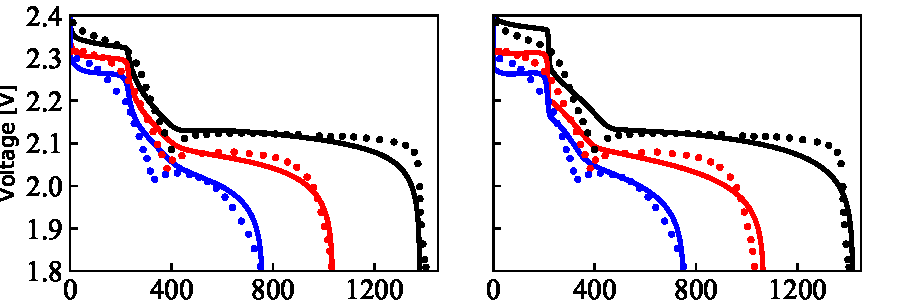
\includegraphics[width=\textwidth]{Figures/Vcell_Andrei_data.pdf}
    \caption{Comparison of the lithiated cascade mechanism and experimental data taken from Andrei \textit{et al} \cite{ANDREI2018469} at 0.1C, 0.5C, and 1C.}
    \label{fig:lithiatedcascadevalidation}
\end{figure}
\end{center}

\subsection{Mechanism comparison}

Figure \ref{fig:mechanismcomparisonvoltage} shows the comparison of discharge voltage for all of the mechanisms implemented. We see that the mechanisms are all relatively close to each other at 0.1C, but quickly diverge at higher C-rates most likely due to kinetic limitations. This highlights one of the most important aspects of modeling sulfur cathodes, which is that both species thermodynamics as well as kinetic parameters are critical to properly model this system on a continuum level. Another feature to notice is between the lithiated and non-lithiated mechanisms, the lithiated mechanism seems to have a smoother transition from the uppper voltage plateau to the lower. This is likely understood by the results shown in figure \ref{fig:mechanismcomparisonconcentration} which shows the species concentrations for each mechanism at 0.1C discharge. When comparing the concentrations in the lithiated mechanism versus the non-lithiated mechanism, while the profiles are similar, they show concentration gradients in the lithiated mechanism compared to the non-lithiated mechanism, which seems to show little or no spatial concentration gradients of the polysulfide species. This presence of concentration gradients may have a smoothing effect on the discharge voltage due to the relationship between polysulfide concentrations and the cell voltage. 

Another aspect of note, particularly between the lithiated and non-lithiated mechanisms, is although their voltages are very similar, the species profiles are different. This is especially noticeable in the magnitude that the concentration of Li$_2$S$_4$/S$_4^{2-}$ and Li$_2$S$_6$/S$_6^{2-}$ reach as well as the different profile of Li$_2$S$_2$/S$_2^{2-}$. 

\begin{center}
\begin{figure}
    \centering
    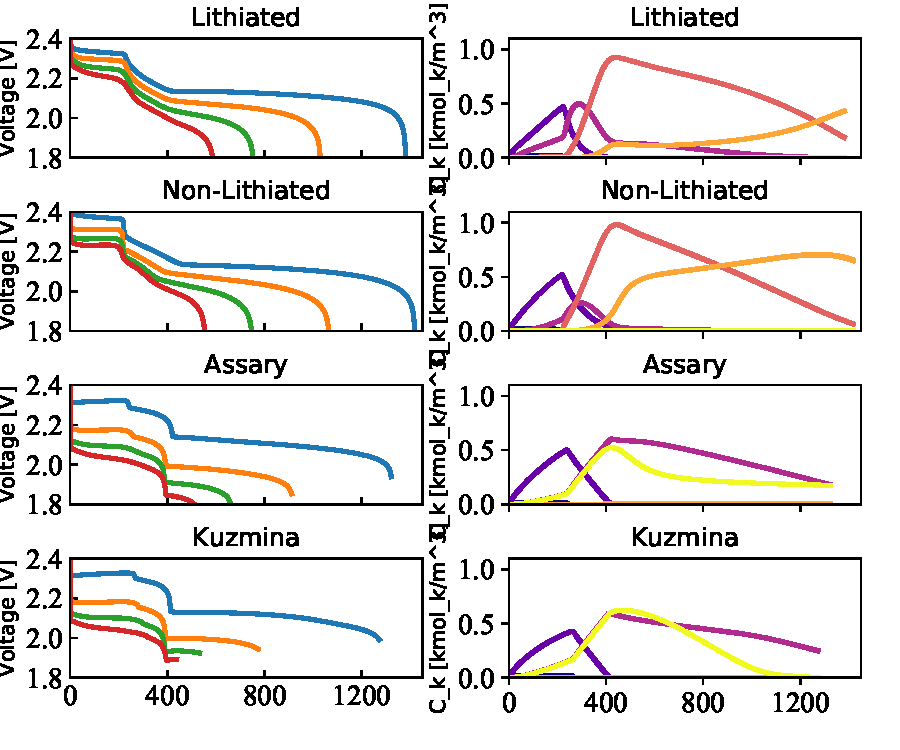
\includegraphics[width=\textwidth]{Figures/Vcell_mech_comp.pdf}
    \caption{Here we are comparing two models based on atomistically determined thermodynamics for intermediate species and two models derived from past continuum level models in the literature. They are being compared at 0.1C, 0.5C, 1C and 1.5C and with a 65\% porous cathode and 25 $\mu$m separator}
    \label{fig:mechanismcomparisonvoltage}
\end{figure}
\end{center}

\subsection{Cell design}

\begin{center}
\begin{figure}
    \centering
    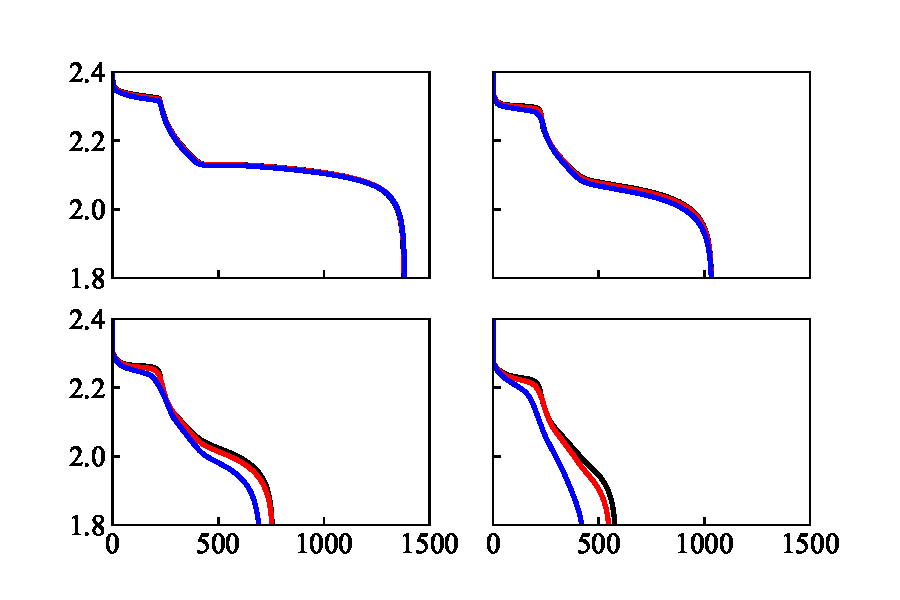
\includegraphics[width=\textwidth]{Figures/Vcell_25um_sep.pdf}
    \caption{Cell voltage for varying porosity at 0.1C, 0.5C, 1C, and 1.5C with a 25 $\mu$m separator. These results agree qualitatively with the literature in that decreasing porosity tends to lead to lower cutoff voltages.}
    \label{fig:porositystudy25umsep}
\end{figure}
\end{center}


\begin{figure}
    \centering
    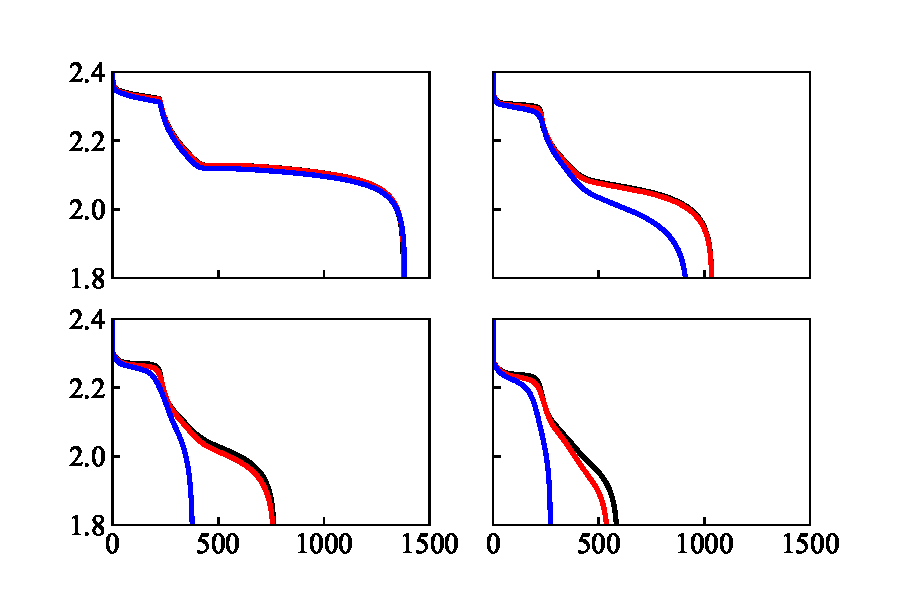
\includegraphics[width=\textwidth]{Figures/Vcell_10um_sep.pdf}
    \caption{Cell voltage for varying porosity at 0.1C, 0.5C, 1C, and 1.5C with a 10 $\mu$m separator. This is a rather thin separator compared to what is commonly used; however, because gravimetric capacity is one of the benefits of Li-S cells, if thinner separators could be used it's one way to trim "dead" material. We see here though that this could affect performance at lower C-rates than with thicker separators.}
    \label{fig:porositystudy10umsep}
\end{figure}

\begin{figure}
    \centering
    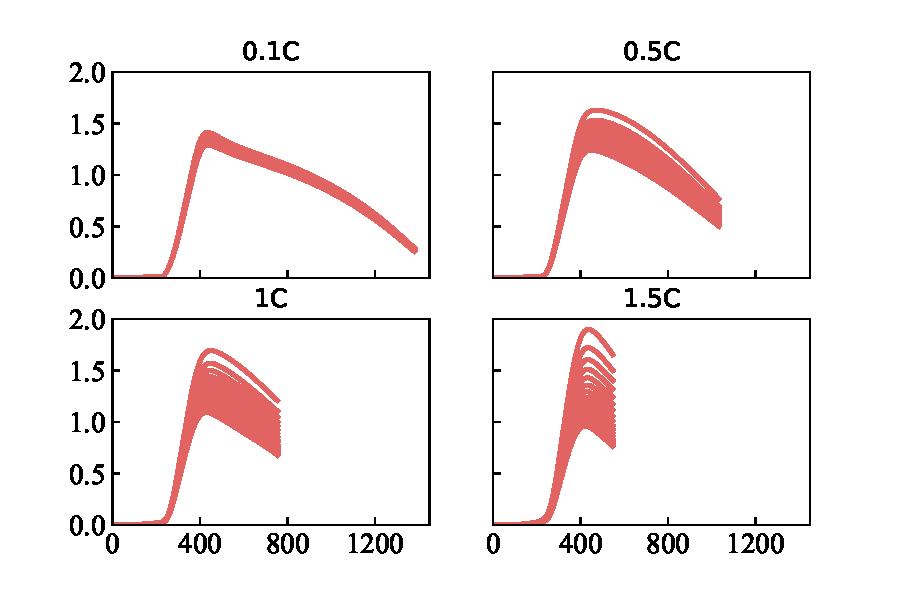
\includegraphics[width=\textwidth]{Figures/Ck_Li2S4.pdf}
    \caption{Comparison of Li2S4 concentration at 0.1C, 0.5C, 1C, and 1.5C with a 25 $\mu$m separator and 65\% cathode porosity.}
    \label{fig:speciescomparisonLi2S4}
\end{figure}

\begin{figure}
    \centering
    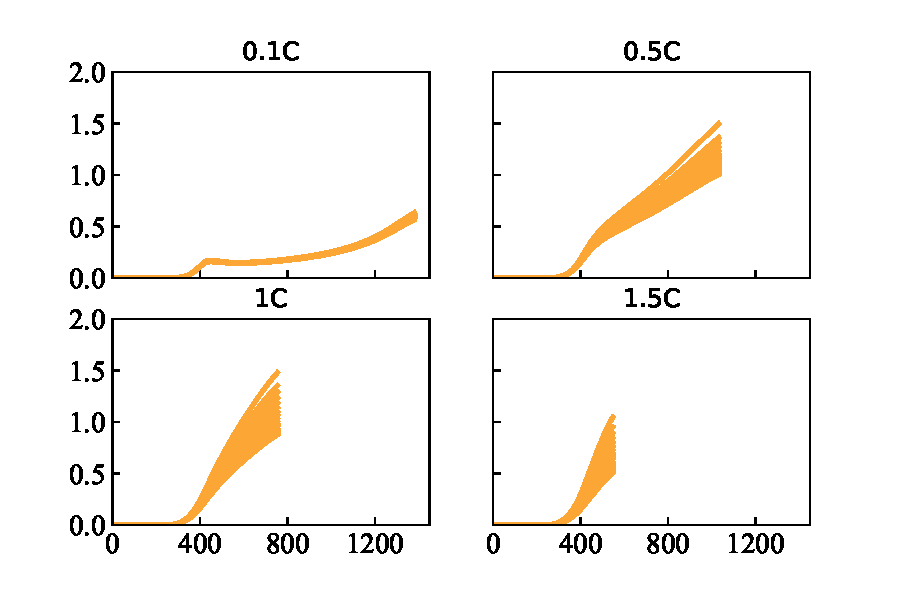
\includegraphics[width=\textwidth]{Figures/Ck_Li2S2.pdf}
    \caption{Comparison of Li2S2 concentration at 0.1C, 0.5C, 1C, and 1.5C with a 25 $\mu$m separator and 65\% cathode porosity}
    \label{fig:speciescomparisonLi2S2}
\end{figure}

\begin{figure}
    \centering
    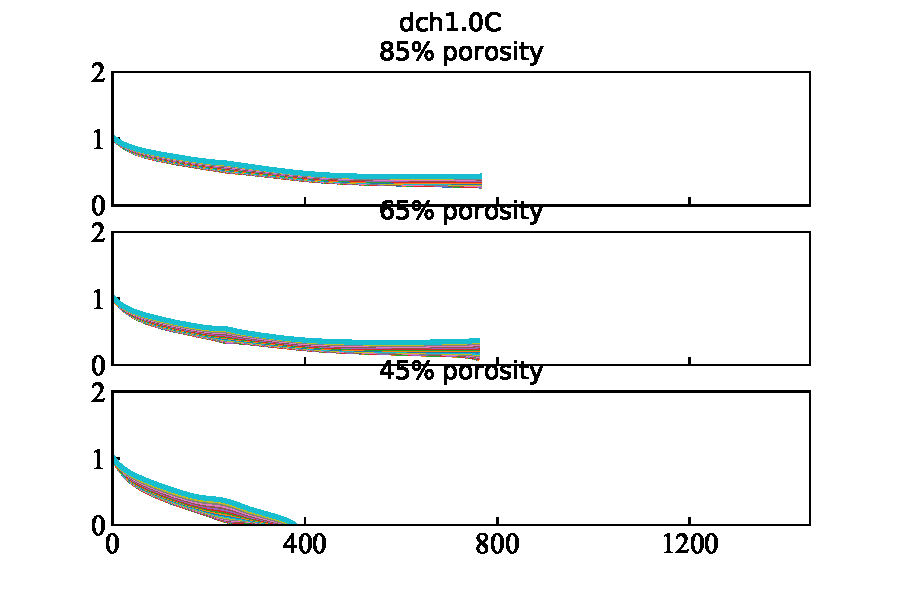
\includegraphics[width=\textwidth]{Figures/C_Lipdch1.0C.pdf}
    \caption{Li+ concentration at varying porosity, 1C discharge, and a 10 $\mu$m separator. This shows with a thin separator the Li+ concentration is depleted.}
    \label{fig:Liconc10umsep}
\end{figure}

\begin{figure}
    \centering
    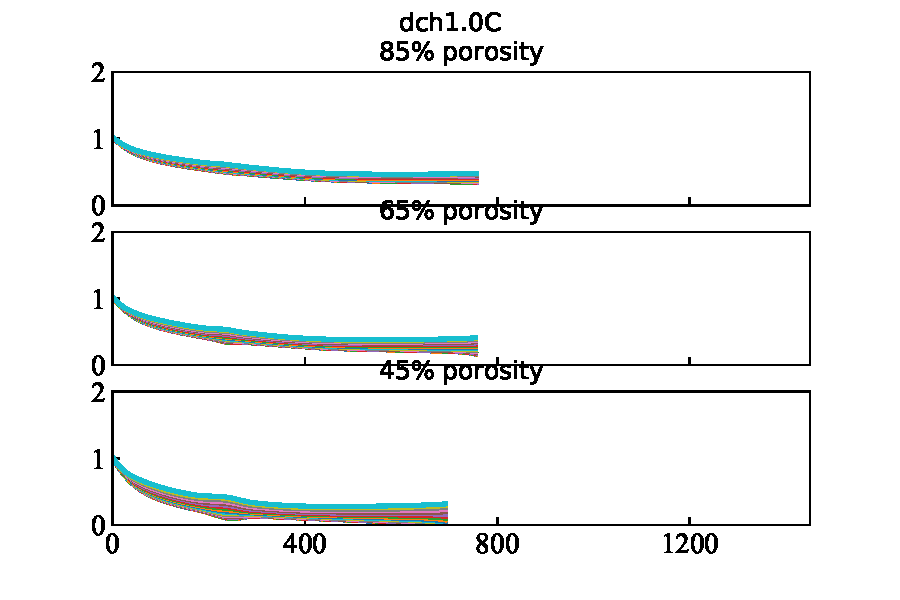
\includegraphics[width=\textwidth]{Figures/C_Lip_25um_dch1.0C.pdf}
    \caption{Li+ concentration in the cathode at varying porosity, 1C discharge, and a 25 $\mu$m separator. With a thicker separator (and more electrolyte volume that it provides) the Li+ isn't fully depleted as with the thinner separator.}
    \label{fig:Liconc25umsep}
\end{figure}

\begin{figure}
    \centering
    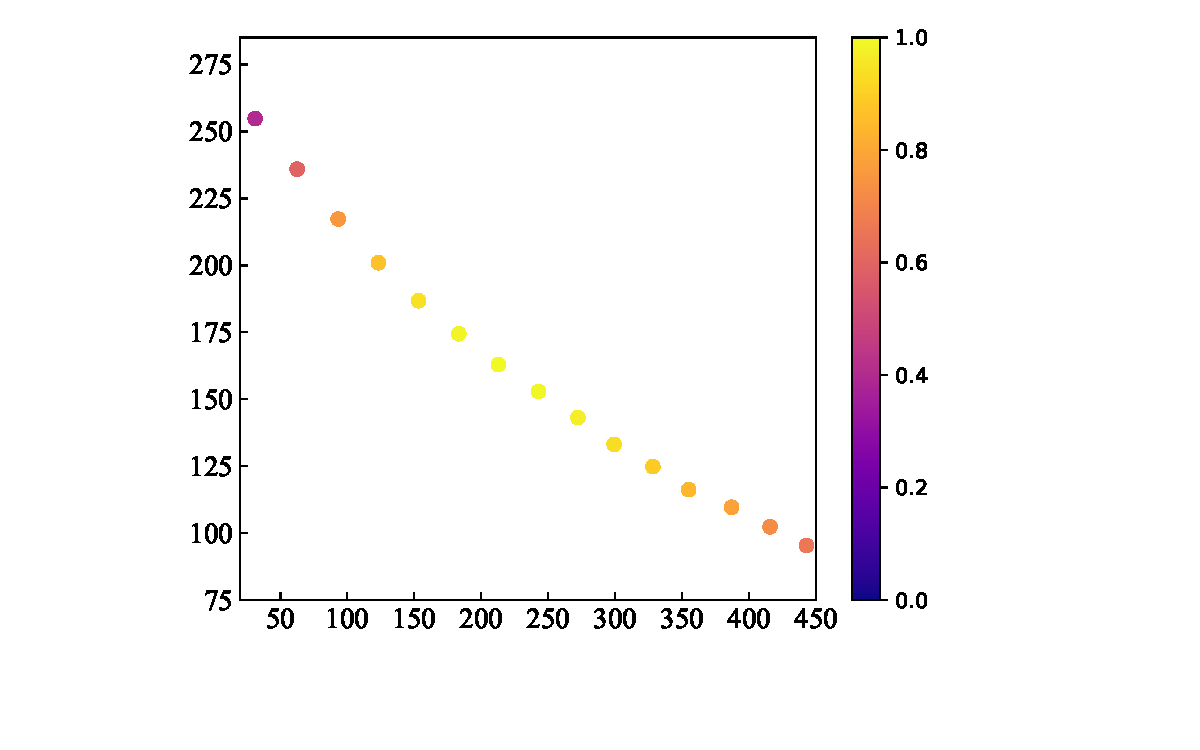
\includegraphics[width=\textwidth]{Figures/Ragone_65pct25um.pdf}
    \caption{Ragone plot showing energy density vs. power density of a 65\% porous cathode with a 25 $\mu$m separator}
    \label{fig:ragone25umsep}
\end{figure}

\begin{figure}
    \centering
    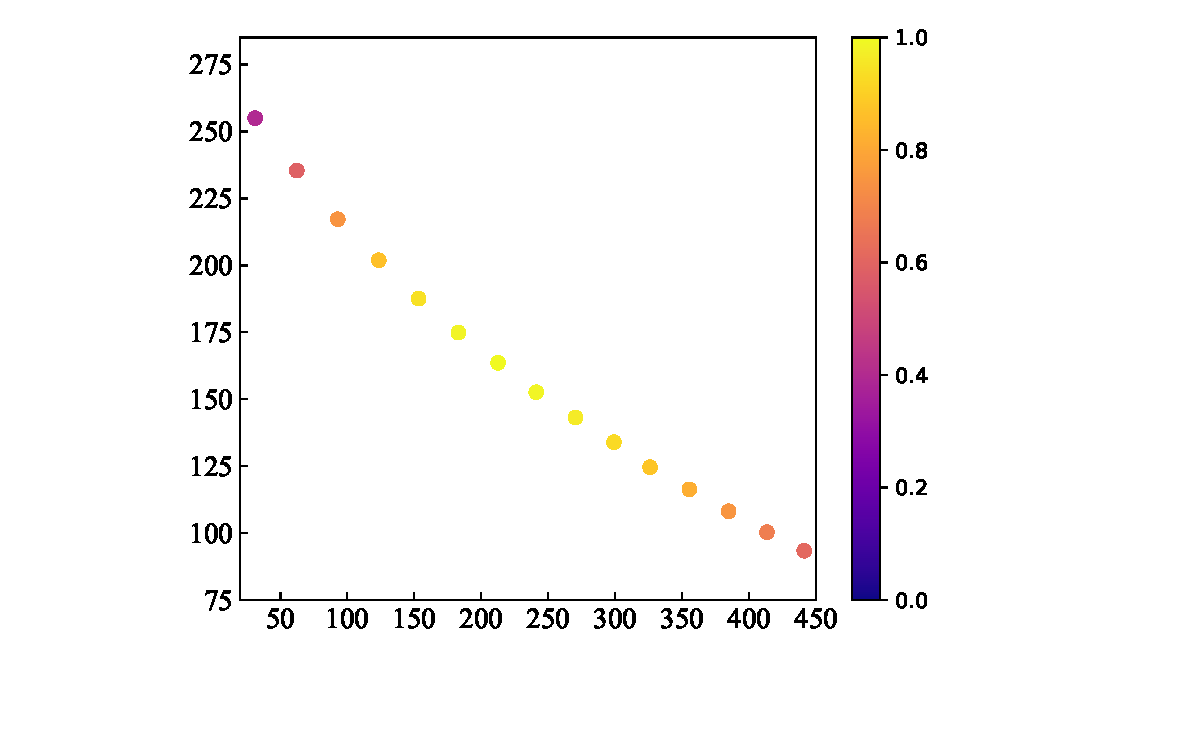
\includegraphics[width=\textwidth]{Figures/Ragone_65pct10um.pdf}
    \caption{Ragone plot showing energy density vs. power density of a 65\% porous cathode with a 10 $\mu$m separator}
    \label{fig:ragone10umsep}
\end{figure}

\newpage

Figures to include:
\begin{itemize}
        \item Verification, Validation, and comparison
        \begin{itemize}
        \item Fig S1 Bessler mech and geom. voltage vs. capacity
        \item \sout{Fig 1 Lithiated V vs. cap at 0.1, 0.5, 1.0C compared to Andrei data}
        \item \sout{Fig 2 Lithiated, non-lithiated, Assary, and Kuzmina V vs. cap (sub-figs for a few C-rates)}
        \item \sout{Fig 3 Lithiated, non-lithiated, Assary, and Kuzmina Conc. vs. cap (sub-figs for mech)}
        \item Compare surface area models?
    \end{itemize}
    \item Single model results - Lithiated cascade
    \begin{itemize}
        \item \sout{Fig 4 Voltage profile for varying cathode porosity at 25 $\mu$m separator}
        \item \sout{Fig 5 voltage profile for varying cathode porosity at 10 $\mu$m separator}
        \item \sout{Fig 6 species profiles as function of C-rate}
        \item Fig 7 species gradient for prominent species as function of C-rate
        \item \sout{Fig 8 Comparison of Li+ concentration gradient for varying porosity at 10 $\mu$m separator}
        \item \sout{Fig 9 Ragone plot for 65\% porous cathode and 25 $\mu$m separator}
        \item \sout{Fig 10 Ragone plot for 65\% porous cathode and 10 $\mu$m separator}
    \end{itemize}
\end{itemize}



%\begin{center}
%\begin{figure}
%    \centering
%    \includegraphics[width=\textwidth]{}
%    \caption{Validation of the lithiated cascade %mechanism versus experimental data.}
%    \label{fig:lithiatedcascadevalidation}
%\end{figure}
%\end{center}

%Validate:
%\begin{itemize}
%    \item As a function of C-rate (charge-discharge)
%    \item Versus Porter's electrolyte data.
%    \item Sensitivity plots.
%\end{itemize}

%\subsection{The Importance of Physical Chemistry %Validation Data}
%\begin{itemize}
%    \item Compare the three mechanisms)
%\end{itemize}


%\subsection{The Impact of Species Solubility on Li-S %Battery Design}
%\subsubsection{Optimizing Power and Energy Density}
%\begin{itemize}
%    \item     Ragone plot
%\end{itemize}
%\subsubsection{Cation Selective Membranes for %Polysulfide Shuttle Mitigation}
%\begin{itemize}
%    \item    Put a ``screening efficiency" at the %cathode/separator boundary.  Observe impact on local %concentrations.  This may need a bit more work--the %model doesn't currently track shuttling current--so %we'll need to decide if it is worth including in this %paper, or saving for later.
%\end{itemize}





%===============================================================%
%                      CONCLUSIONS
%===============================================================%
\section{Conclusions}


\newpage
\bibliography{mybib}
\newpage



\end{document}